\documentclass[xetex,mathserif,serif,aspectratio=169]{beamer}

\usepackage{xltxtra}
\usepackage{color}
\usepackage{url}
\usepackage{listings}
\usepackage{fontspec}
\usepackage{geometry}
\usepackage{lastpage}
\usepackage{fancyhdr}
\usepackage{amsmath}
\usepackage{amsthm}
\usepackage{amssymb}
\usepackage{blkarray}
\usepackage{multicol}
\usepackage{relsize}
\usepackage{listings}
\usepackage{xunicode}
\usepackage{xltxtra}
\usepackage{color}
\usepackage{url}
\usefonttheme[onlymath]{serif}

\definecolor{solarized@base03}{HTML}{002B36}
\definecolor{solarized@base02}{HTML}{073642}
\definecolor{solarized@base01}{HTML}{586e75}
\definecolor{solarized@base00}{HTML}{657b83}
\definecolor{solarized@base0}{HTML}{839496}
\definecolor{solarized@base1}{HTML}{93a1a1}
\definecolor{solarized@base2}{HTML}{EEE8D5}
\definecolor{solarized@base3}{HTML}{FDF6E3}
\definecolor{solarized@yellow}{HTML}{B58900}
\definecolor{solarized@orange}{HTML}{CB4B16}
\definecolor{solarized@red}{HTML}{DC322F}
\definecolor{solarized@magenta}{HTML}{D33682}
\definecolor{solarized@violet}{HTML}{6C71C4}
\definecolor{solarized@blue}{HTML}{268BD2}
\definecolor{solarized@cyan}{HTML}{2AA198}
\definecolor{solarized@green}{HTML}{859900}
\definecolor{yaleblue}{HTML}{0E4C92}

\newcommand{\yellow}[1]{\textcolor{solarized@yellow}{#1}}
\newcommand{\orange}[1]{\textcolor{solarized@orange}{#1}}
\newcommand{\red}[1]{\textcolor{solarized@red}{#1}}
\newcommand{\magenta}[1]{\textcolor{solarized@magenta}{#1}}
\newcommand{\violet}[1]{\textcolor{solarized@violet}{#1}}
\newcommand{\blue}[1]{\textcolor{solarized@blue}{#1}}
\newcommand{\cyan}[1]{\textcolor{solarized@cyan}{#1}}
\newcommand{\green}[1]{\textcolor{solarized@green}{#1}}
\newcommand{\yblue}[1]{\textcolor{yaleblue}{#1}}
\newcommand{\base}[1]{\textcolor{solarized@base01}{#1}}


\defaultfontfeatures{Mapping=tex-text}
\hypersetup{pdfstartview={FitH}}

\newcommand{\old}[1]{\fontspec[Alternate=1,Ligatures={Common}]{Hoefler Text}\fontsize{18pt}{30pt}\selectfont #1}%
\newcommand{\oldA}[1]{\fontspec[Alternate=1,Ligatures={Common, Rare}]{Hoefler Text}\fontsize{12pt}{15pt}\selectfont #1}%
\newcommand{\oldB}[1]{\fontspec[Ligatures={Common}]{Didot}\fontsize{12pt}{15pt}\color{solarized@base02}\selectfont #1}%
\newcommand{\tfont}[1]{\fontspec[Alternate=1,Ligatures={Common}]{Hoefler Text}\fontsize{12pt}{20pt}\selectfont #1}%
\newcommand{\dfont}[1]{\fontspec[Ligatures={Common}]{Didot}\fontsize{12pt}{12pt}\selectfont #1}%

\setbeamerfont{title}{family=\old}
\setbeamerfont{author}{family=\tfont}%
\setbeamerfont{frametitle}{family=\oldA}
\setbeamerfont{date}{family=\dfont}

\setbeamertemplate{navigation symbols}{}
\setbeamertemplate{footline}[text line]{%
  \parbox{0.99\linewidth}{
    \normalsize\vspace*{-24pt}\hfill{\color{solarized@base00}\insertframenumber/\inserttotalframenumber}
  }
}


\setlength{\parindent}{0pt}
\setlength{\parskip}{12pt}

\setbeamercolor{structure}{bg=solarized@base3, fg=solarized@base02}
\setbeamercolor{titlelike}{fg=solarized@cyan}
\setbeamercolor{title}{fg=solarized@blue}
\setbeamercolor{subtitle}{fg=solarized@magenta}
\setbeamercolor{alerted text}{fg=orange}
\setbeamercolor{itemize}{fg=solarized@base02}
\setbeamercolor{background canvas}{bg=solarized@base3}
\setbeamercolor{enumerate subitem}{fg=solarized@base02}

\newcommand{\minimize}{\mathop{\mathrm{minimize}}}
\newcommand{\argmin}{\mathop{\mathrm{arg\,min}}}
\newcommand{\argmax}{\mathop{\mathrm{arg\,max}}}
\newcommand{\st}{\mathop{\mathrm{subject\,\,to}}}



\begin{document}

%%%%%%%%%%%%%%%%%%%%%%%%%%%%%%%%%%%%%%%%%%%%%%%%%%%
\begin{frame}[fragile] \frametitle{} \oldB \small

\vfill

{\fontsize{0.7cm}{0cm}\selectfont Lecture 03 \\\vspace{0.2cm} Linear classification methods II}\\\vspace{0.5cm}
25 January 2016

\vspace{2cm}

\begin{minipage}{0.6\textwidth}
Taylor B. Arnold \\
Yale Statistics \\
STAT 365/665
\end{minipage}
\hfill
\begin{minipage}{0.3\textwidth}\raggedleft

\includegraphics[scale=0.3]{../yale-logo.png}
\end{minipage}%

\end{frame}

%%%%%%%%%%%%%%%%%%%%%%%%%%%%%%%%%%%%%%%%%%%%%%%%%%%
\begin{frame}[fragile] \frametitle{} \oldB \small

\begin{itemize}
\item Office hours
\begin{itemize}
\item Taylor Arnold -- Mondays, 13:00 - 14:15, HH 24, Office 203 (by appointment)
\item Yu Lu -- Tuesdays, 10:00-12:00, HH 24, Library
\item Jason Klusowski -- Thursdays, 19:00-20:30, HH 24
\end{itemize}
\item Problem set \#2 - Posted, on ClassesV2, updated datasets (as of 2015-01-23)
\item Enrollment\ldots
\end{itemize}

\end{frame}

%%%%%%%%%%%%%%%%%%%%%%%%%%%%%%%%%%%%%%%%%%%%%%%%%%%
\begin{frame}[fragile] \frametitle{} \oldB \small

\begin{center}
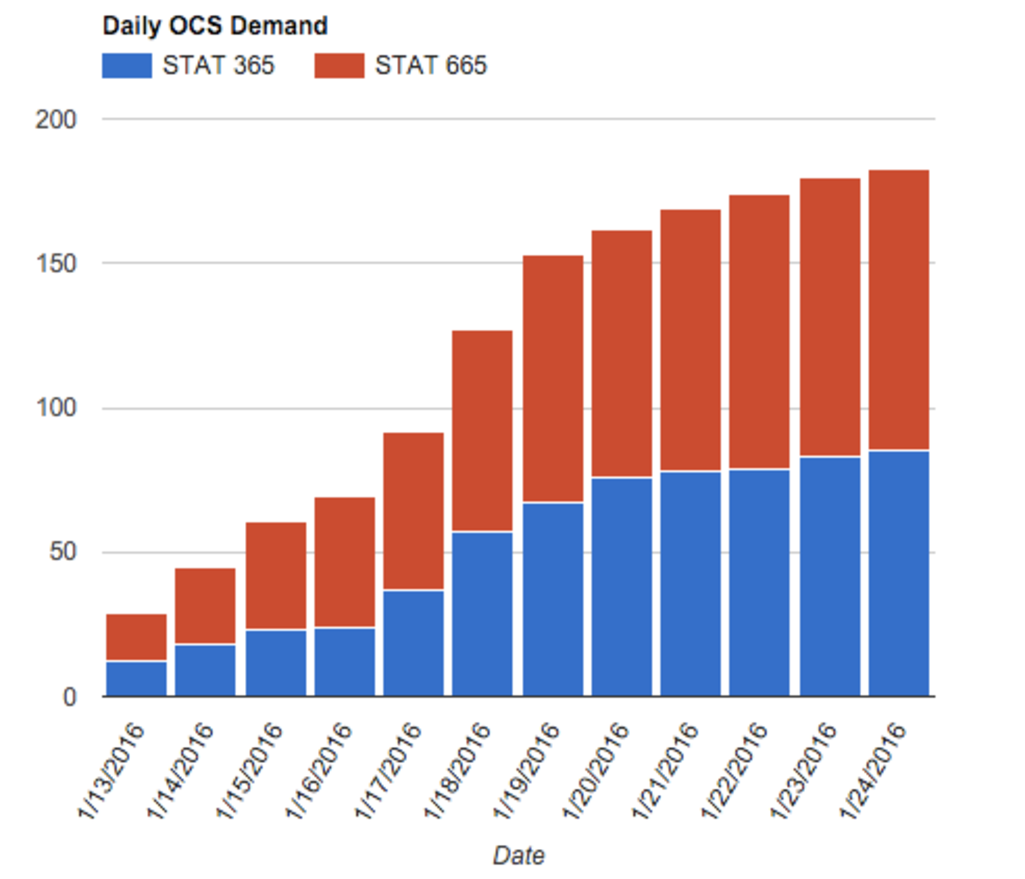
\includegraphics[width=0.7\textwidth]{img/stat665.pdf}
\end{center}

\end{frame}

%%%%%%%%%%%%%%%%%%%%%%%%%%%%%%%%%%%%%%%%%%%%%%%%%%%
\begin{frame}[fragile] \frametitle{} \oldB \small

Last class we considered solutions to the
\blue{$1$-dimensional non-parametric regression} problem.
Specifically, we considered observing $n$ pairs $(x_i,y_i)$ such
that:
\begin{align*}
y_i &= g(x_i) + \epsilon_i
\end{align*}
For an unknown function $g$ and random variable $\epsilon_i$, where the mean
of the random variable is zero.

The goal was to estimate the function $g$.

\end{frame}

%%%%%%%%%%%%%%%%%%%%%%%%%%%%%%%%%%%%%%%%%%%%%%%%%%%
\begin{frame}[fragile] \frametitle{} \oldB \small

The specific methods we used to do this were:

\begin{enumerate}
\item k-nearest neighbors (knn)
\item kernel smoothing (Nadaraya-Watson estimator)
\item linear regression (OLS)
\item local regression (LOESS)
\end{enumerate}

\end{frame}

%%%%%%%%%%%%%%%%%%%%%%%%%%%%%%%%%%%%%%%%%%%%%%%%%%%
\begin{frame}[fragile] \frametitle{} \oldB \small

\yblue{\textbf{Linear smoothers}}

How are these four techniques all related?\pause

All of them can be written as:
\begin{align*}
\widehat{y}_{new} &= \widehat{g}(x_{new}) \\
&= \sum_i w_i y_i
\end{align*}
Where the weights $w_i$ depend only on the values $x_i$ (and $x_{new}$)
and not on the values of $y_i$.

\pause Anything that can be written in this form is called
a \blue{linear smoother}.

\end{frame}

%%%%%%%%%%%%%%%%%%%%%%%%%%%%%%%%%%%%%%%%%%%%%%%%%%%
\begin{frame}[fragile] \frametitle{} \oldB \small

\yblue{\textbf{Linear smoothers, cont.}}

For example, in the case of \magenta{knn}, the weights are $\frac{1}{k}$
for the $k$ closest values and $0$ for the rest of them.

\pause We have already seen the weights for the \magenta{kernel smoother} by
its definition.

\pause The weights for \magenta{ordinary least squares} are given by the matrix
product ($X$ is the data matrix from basis expansion of the inputs):
\begin{align*}
w &= X_{new} (X^t X)^{-1} X^t
\end{align*}

\pause And \magenta{LOESS} is simply a sample weighted variant of the least squares:
\begin{align*}
w &= X_{new} (X^t D X)^{-1} X^t D
\end{align*}
For a diagonal matrix of weights $D = \text{diag}\left(\phi(||x_{new} - x_i||_2)\right)$.

\end{frame}

%%%%%%%%%%%%%%%%%%%%%%%%%%%%%%%%%%%%%%%%%%%%%%%%%%%
\begin{frame}[fragile] \frametitle{} \oldB \small

\yblue{\textbf{Linear smoothers, cont.}}

There is a substantial amount of theory regarding the
class of linear smoothers.

If you are interested in more, the best first reference
is the following text (you can download a free pdf):
\begin{quote}
Cosma Rohilla Shalizi. \textit{Advanced Data Analysis from an Elementary Point of View}. Book in preparation. \url{http://www.stat.cmu.edu/~cshalizi/ADAfaEPoV/}.
\end{quote}

\end{frame}

%%%%%%%%%%%%%%%%%%%%%%%%%%%%%%%%%%%%%%%%%%%%%%%%%%%
\begin{frame}[fragile] \frametitle{} \oldB \small

\yblue{\textbf{Computational issues}}

I have not yet talked about how these algorithms should be implemented.
Problem set \#1 asks you to write your own implementation of knn and
kernel smoothing; \blue{brute force} is fine for the assignment, but
can we do better?

\end{frame}

%%%%%%%%%%%%%%%%%%%%%%%%%%%%%%%%%%%%%%%%%%%%%%%%%%%
\begin{frame}[fragile] \frametitle{} \oldB \small

\yblue{\textbf{Computational issues, cont.}}

If we want to classify $m$ new data points, and have $n$ observations in the
original dataset, what is the computational complexity of the brute force
knn or kernel smoother?

\pause We need to construct the entire $m$ by $n$ distance matrix, and so
this takes a total of $\magenta{m\cdot n}$ operations. For a small $m$, this
is actually quite satisfactory. For a larger value of $m$, refitting on the
entire training set for example, this can become prohibitive for large
sample sizes.

\end{frame}


%%%%%%%%%%%%%%%%%%%%%%%%%%%%%%%%%%%%%%%%%%%%%%%%%%%
\begin{frame}[fragile] \frametitle{} \oldB \small

\yblue{\textbf{Computational issues, cont.}}

Consider first sorting the inputs:
\begin{align*}
x_1 \leq x_2 \leq \cdots \leq x_{n-1} \leq x_{n}
\end{align*}
This can be done in $\magenta{O(n \cdot log(n))}$ time.

\pause Using binary search, we can insert a new observation $x_{new}$ into
this sorted sequence in $\magenta{O(log(n))}$ operations:
\begin{align*}
x_{r} \leq x_{new} \leq x_{r+1}
\end{align*}
\pause For knn, we can then look at only the $k$ neighbors less than $x_{new}$
and the $k$ neighbors greater than $x_{new}$. The $k$ nearest neighbors are
guaranteed to be in this set. This only takes $\magenta{2k}$ time.

\pause This implementation takes only \magenta{$O(mk \cdot  \log(n))$} operations to fit new
observations.

\end{frame}

%%%%%%%%%%%%%%%%%%%%%%%%%%%%%%%%%%%%%%%%%%%%%%%%%%%
\begin{frame}[fragile] \frametitle{} \oldB \small

\yblue{\textbf{Computational issues, cont.}}

Now, consider the following intervals:
\begin{align*}
B_q &= \left[ x_{min} + h\cdot(q - 1), \quad x_{min} + h\cdot q \right)
\end{align*}
For some fixed bandwidth $h$. There should be $range(x) / h$ such buckets,
a constant we will define as $N$.

\pause Partitioning the input variables $x_i$ into these
buckets takes only $\magenta{n}$ operations.

\pause If we use kernel smoothing truncated at a distance $h/2$ away from
the mean, we can estimate $\widehat{y_{new}}$ for a new input by only looking
at points inside $2$ of the buckets $B_q$. How long this takes depends on
how evenly distributed the data are across the range of $x$.

\pause If the inputs are evenly spread out over the input space, we can
fit kernel smoothing on $m$ new inputs in $\magenta{O(n + mn/N)}$ time.

\end{frame}


%%%%%%%%%%%%%%%%%%%%%%%%%%%%%%%%%%%%%%%%%%%%%%%%%%%
\begin{frame}[fragile] \frametitle{} \oldB \small

\yblue{\textbf{Computational issues, cont.}}

In one dimension these algorithms are fairly straightforward. We will
continue to discuss how to implement these when the number of dimensions
is larger. Sorting obviously does not work directly; bucketing \textit{can}
for a reasonable number of dimensions but becomes ineffective for large
dimensional spaces.

\end{frame}

%%%%%%%%%%%%%%%%%%%%%%%%%%%%%%%%%%%%%%%%%%%%%%%%%%%
\begin{frame}[fragile] \frametitle{} \oldB \small

\yblue{\textbf{Tuning parameters}}

Last class we spent a while looking at how these four estimators vary with
respect to their tuning parameters.

How do we actually choose the value of the tuning parameter to use a prediction
system?

\end{frame}

%%%%%%%%%%%%%%%%%%%%%%%%%%%%%%%%%%%%%%%%%%%%%%%%%%%
\begin{frame}[fragile] \frametitle{} \oldB \small

\yblue{\textbf{Tuning parameters, cont.}}

There is a lot of theory that establishes asymptotic formulas for the form
of some tuning parameters. For example, the bandwidth in kernel smoothing
should be of the form $O(n^{-1/5})$.

\pause Unfortunately, in almost every case I know of these theoretical results yield
poor results when directly applied to finite samples. We need to instead
estimate the value of the tuning parameter from the data itself.

\end{frame}

%%%%%%%%%%%%%%%%%%%%%%%%%%%%%%%%%%%%%%%%%%%%%%%%%%%
\begin{frame}[fragile] \frametitle{} \oldB \small

\begin{center}
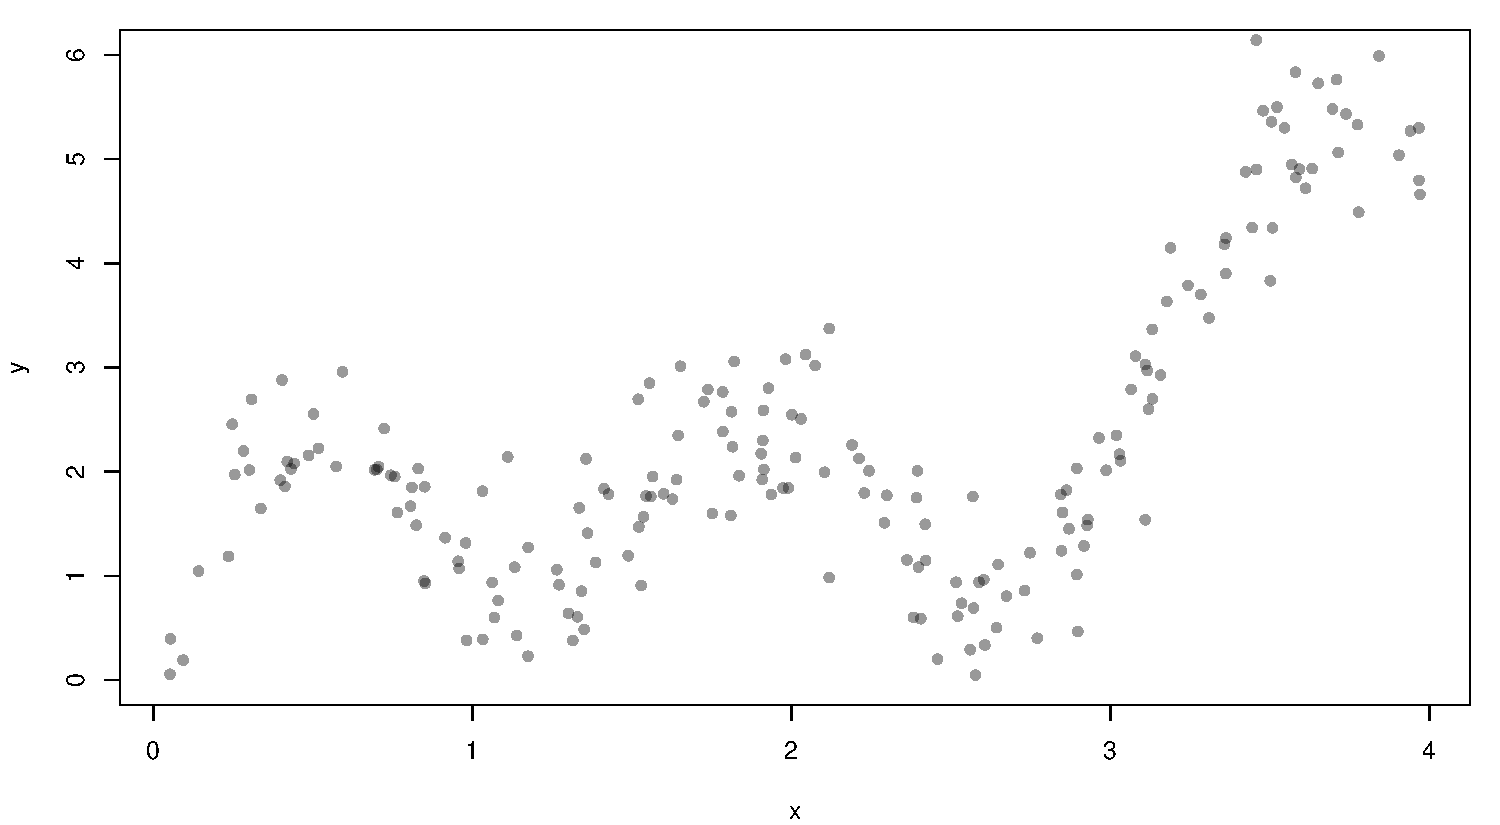
\includegraphics[width=\textwidth]{img/valid1.pdf}
\end{center}

\end{frame}

%%%%%%%%%%%%%%%%%%%%%%%%%%%%%%%%%%%%%%%%%%%%%%%%%%%
\begin{frame}[fragile] \frametitle{} \oldB \small

\begin{center}
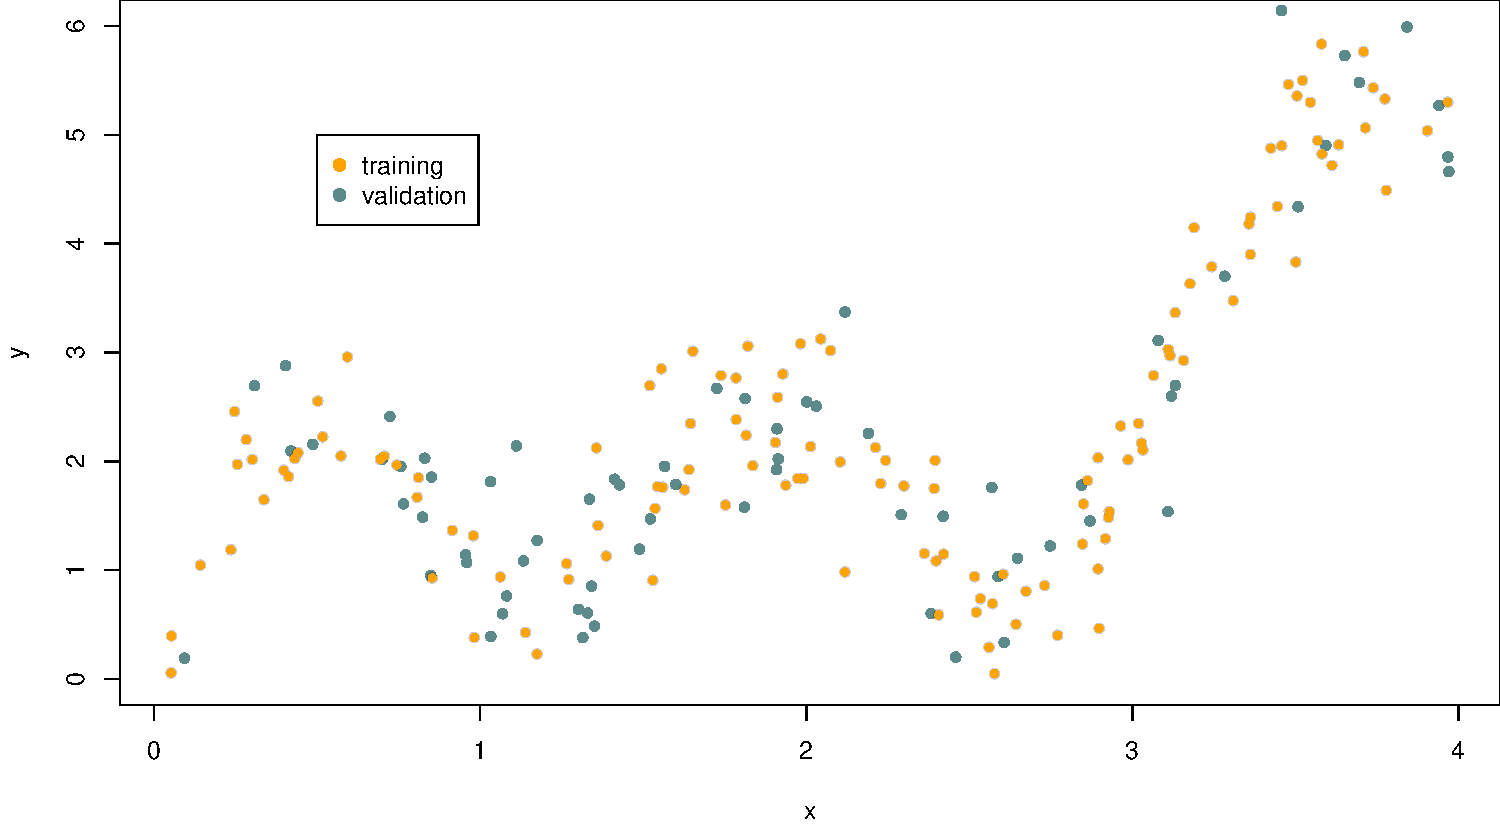
\includegraphics[width=\textwidth]{img/valid2.pdf}
\end{center}

\end{frame}

%%%%%%%%%%%%%%%%%%%%%%%%%%%%%%%%%%%%%%%%%%%%%%%%%%%
\begin{frame}[fragile] \frametitle{} \oldB \small

\begin{center}
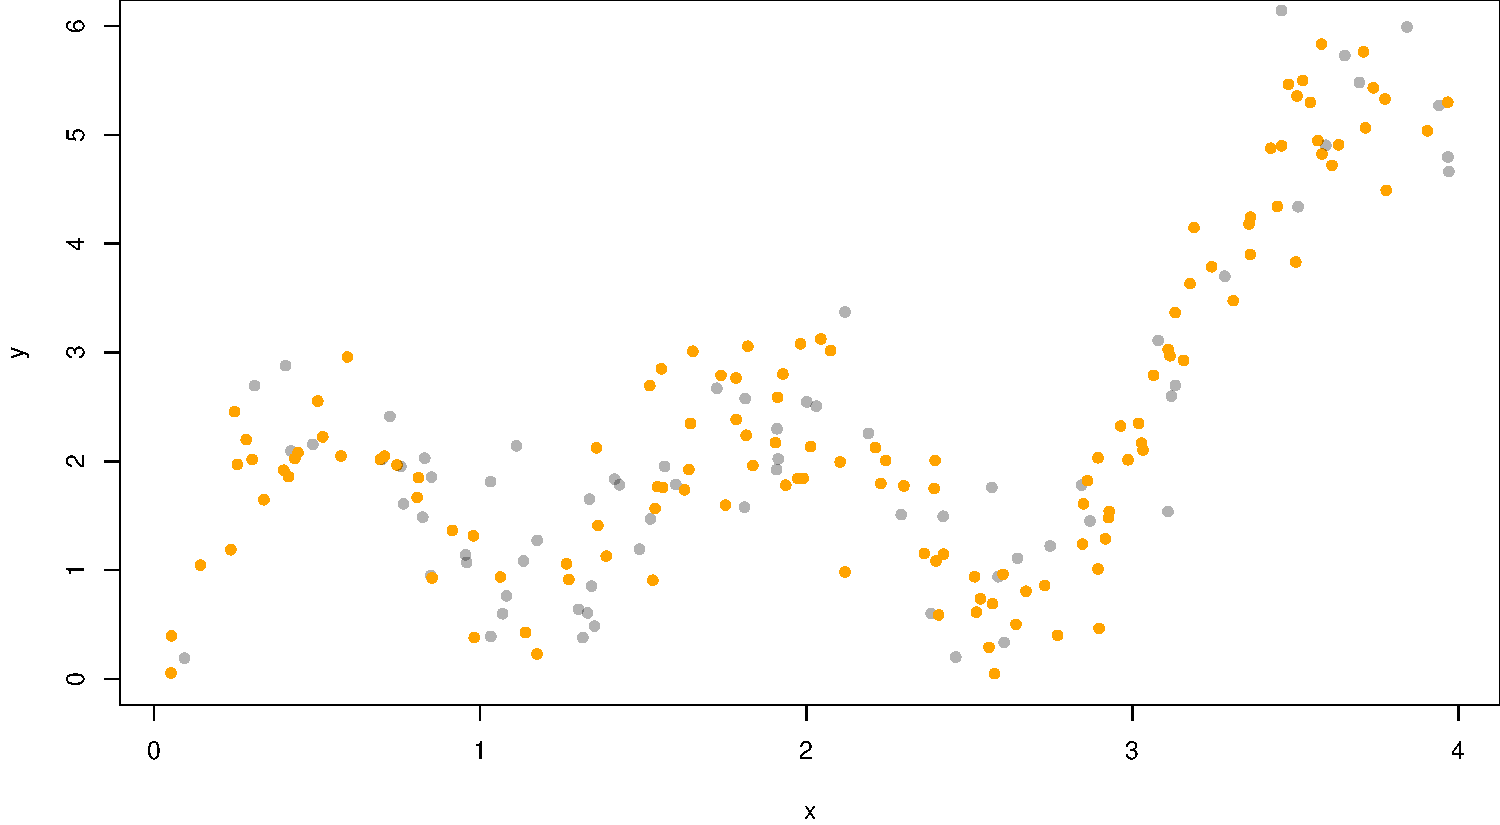
\includegraphics[width=\textwidth]{img/valid3.pdf}
\end{center}

\end{frame}

%%%%%%%%%%%%%%%%%%%%%%%%%%%%%%%%%%%%%%%%%%%%%%%%%%%
\begin{frame}[fragile] \frametitle{} \oldB \small

\begin{center}
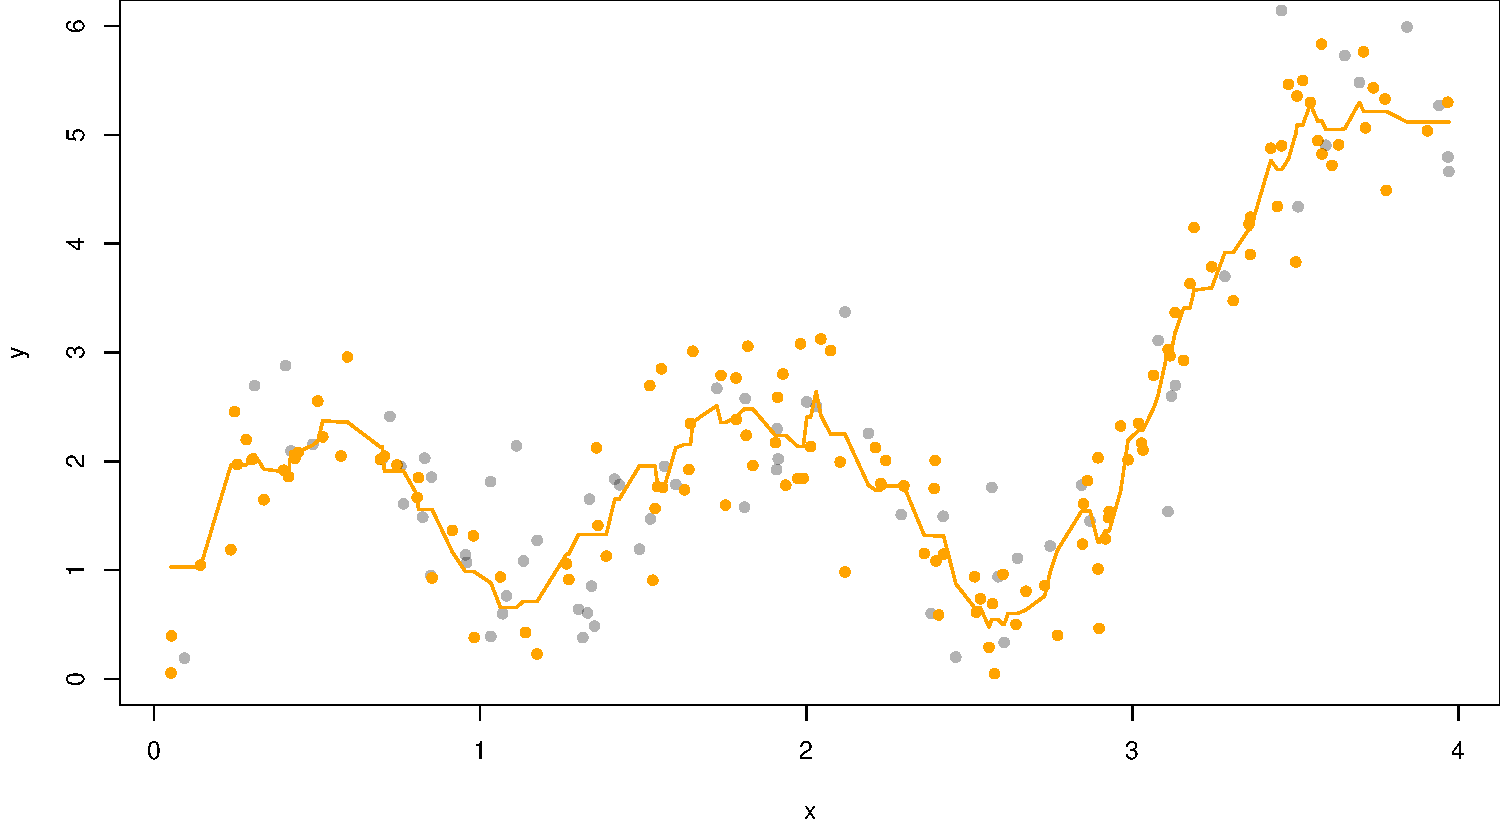
\includegraphics[width=\textwidth]{img/valid4.pdf}
\end{center}

\end{frame}

%%%%%%%%%%%%%%%%%%%%%%%%%%%%%%%%%%%%%%%%%%%%%%%%%%%
\begin{frame}[fragile] \frametitle{} \oldB \small

\begin{center}
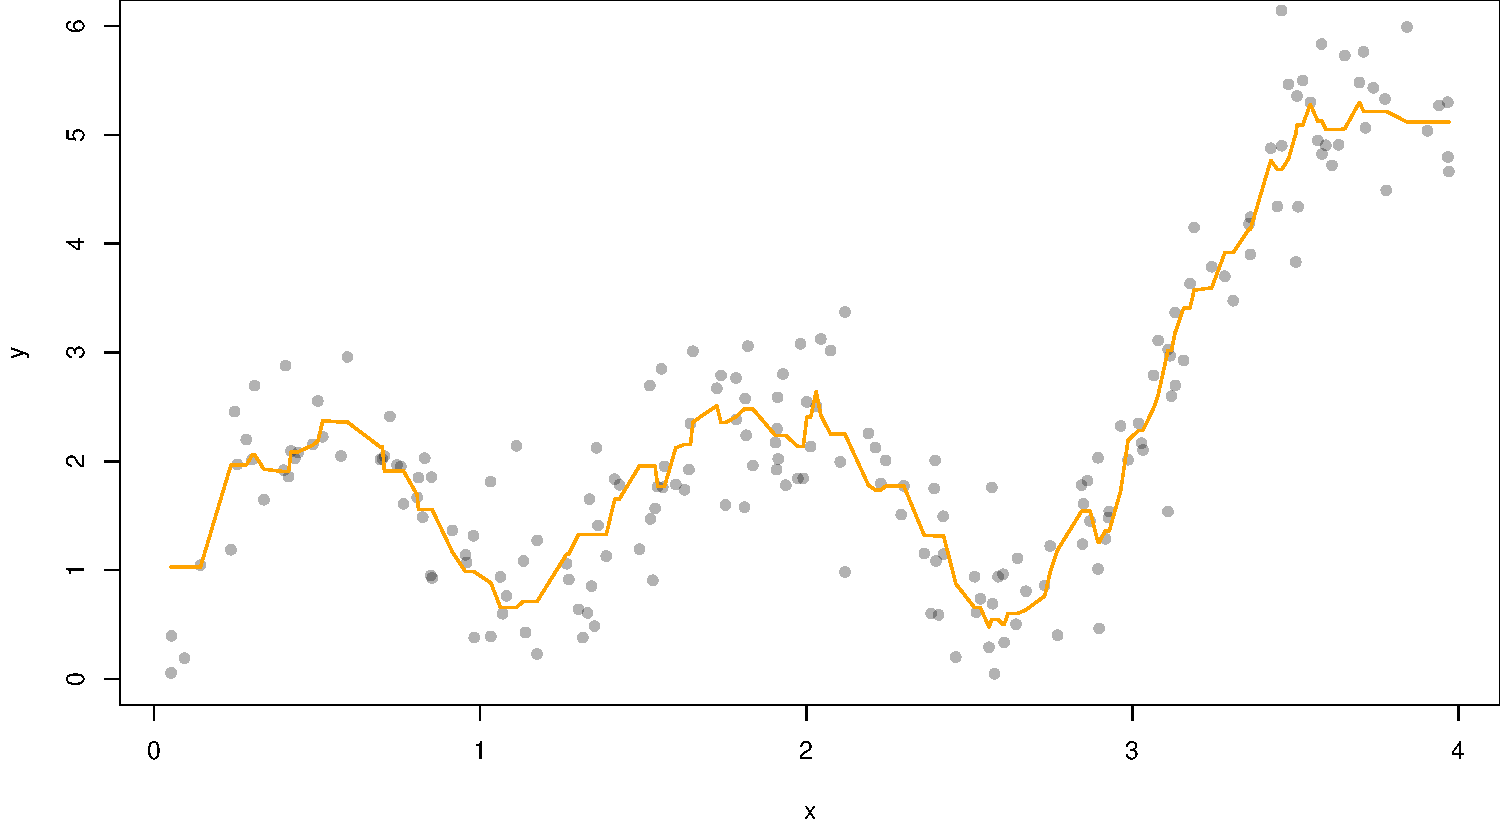
\includegraphics[width=\textwidth]{img/valid5.pdf}
\end{center}

\end{frame}

%%%%%%%%%%%%%%%%%%%%%%%%%%%%%%%%%%%%%%%%%%%%%%%%%%%
\begin{frame}[fragile] \frametitle{} \oldB \small

\begin{center}
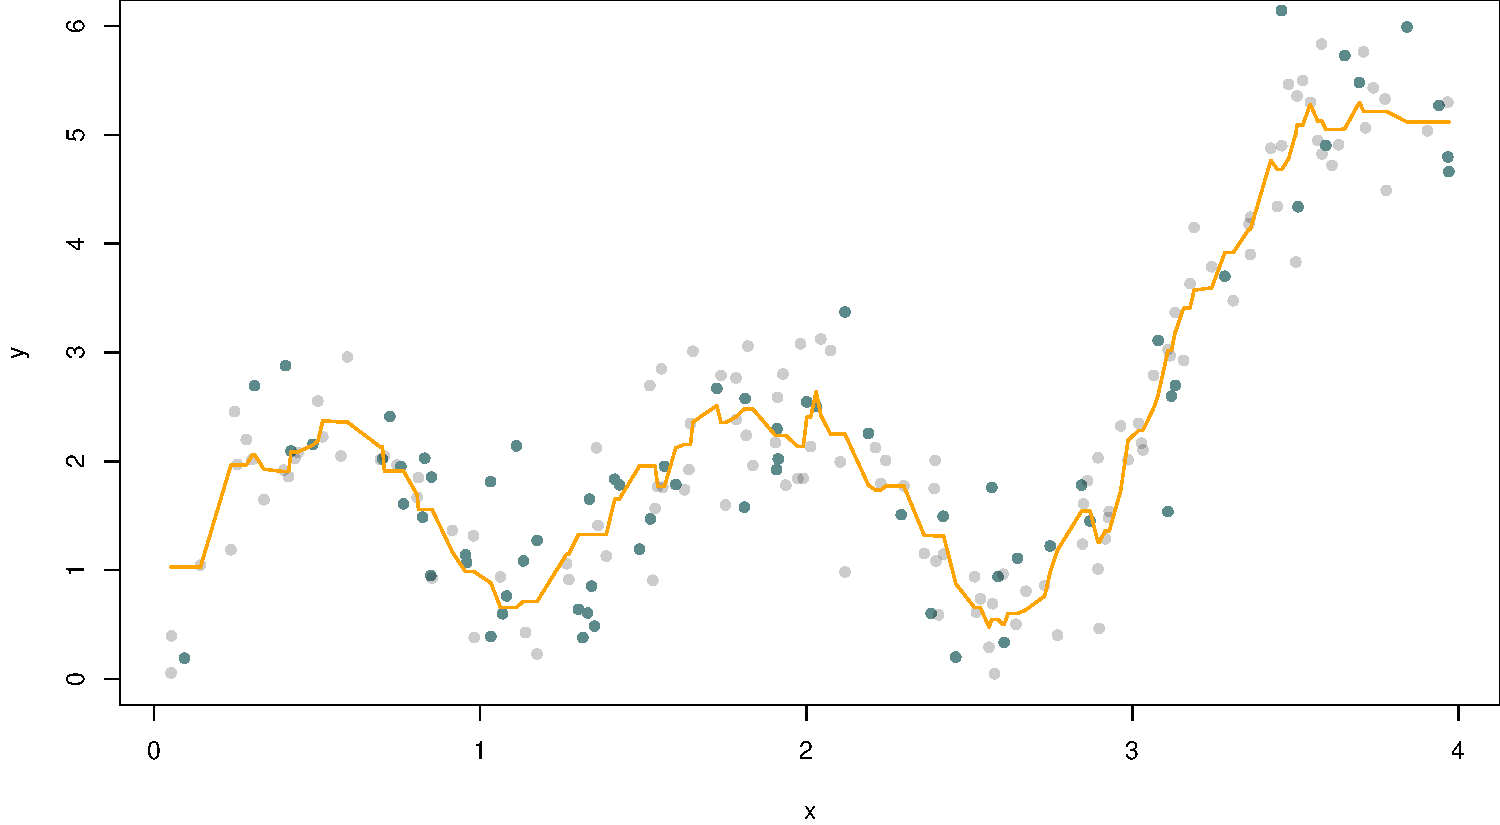
\includegraphics[width=\textwidth]{img/valid6.pdf}
\end{center}

\end{frame}

%%%%%%%%%%%%%%%%%%%%%%%%%%%%%%%%%%%%%%%%%%%%%%%%%%%
\begin{frame}[fragile] \frametitle{} \oldB \small

\begin{center}
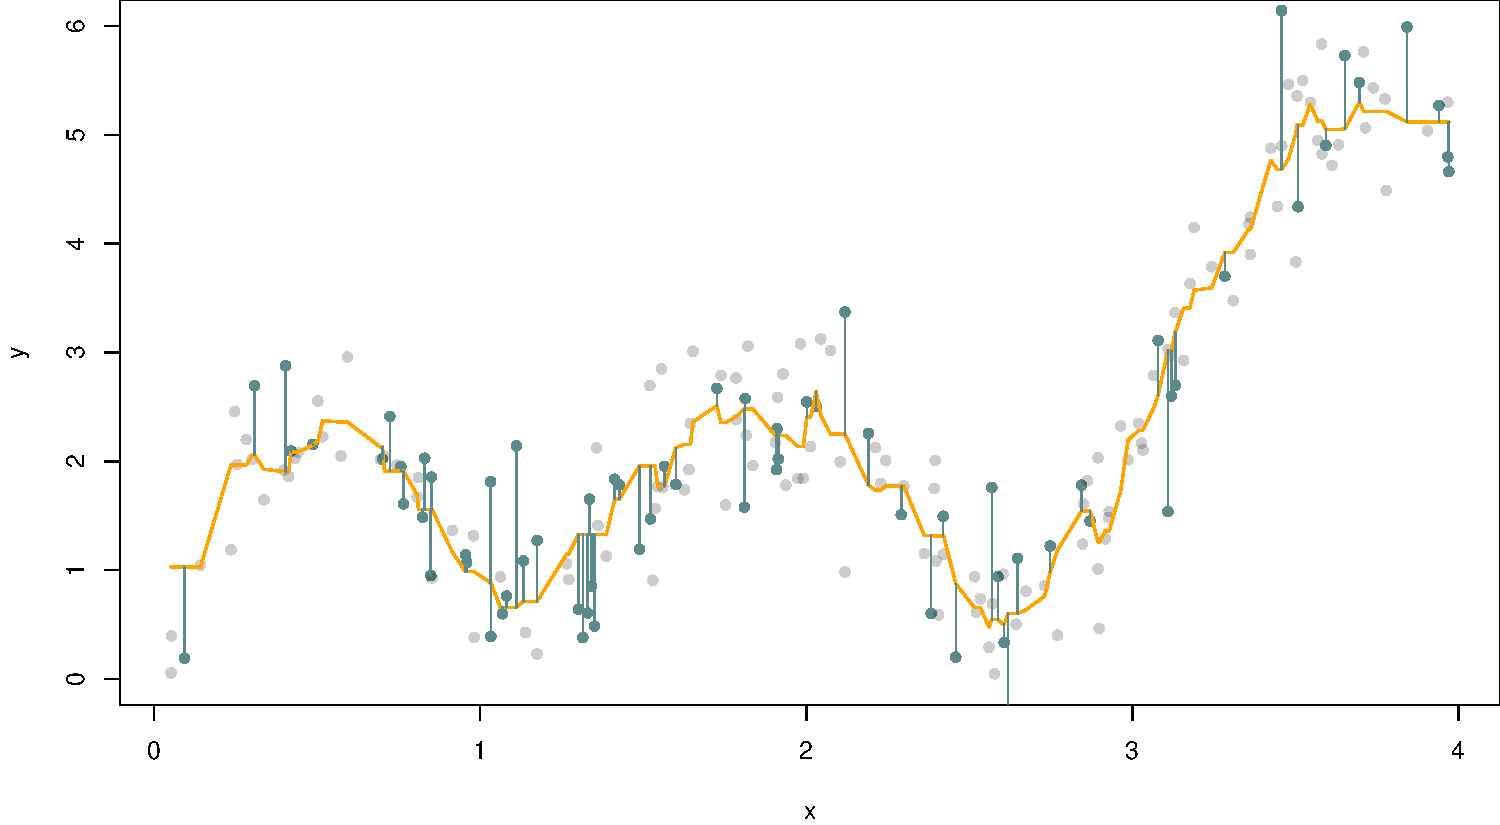
\includegraphics[width=\textwidth]{img/valid7.pdf}
\end{center}

\end{frame}

%%%%%%%%%%%%%%%%%%%%%%%%%%%%%%%%%%%%%%%%%%%%%%%%%%%
\begin{frame}[fragile] \frametitle{} \oldB \small

\yblue{\textbf{Tuning parameters, cont.}}

With this setup, we can now define the mean squared (validation) error:
\begin{align*}
MSE(k) &= \frac{1}{\#\{V\}} \sum_{i \in V} \left(y_i - \widehat{g}_k(x_i) \right)^2
\end{align*}
We can then optimize this function over $k$ (or whatever tuning parameter
is appropriate for the model of choice) to pick the final model.

\end{frame}

%%%%%%%%%%%%%%%%%%%%%%%%%%%%%%%%%%%%%%%%%%%%%%%%%%%
\begin{frame}[fragile] \frametitle{} \oldB \small

\begin{center}
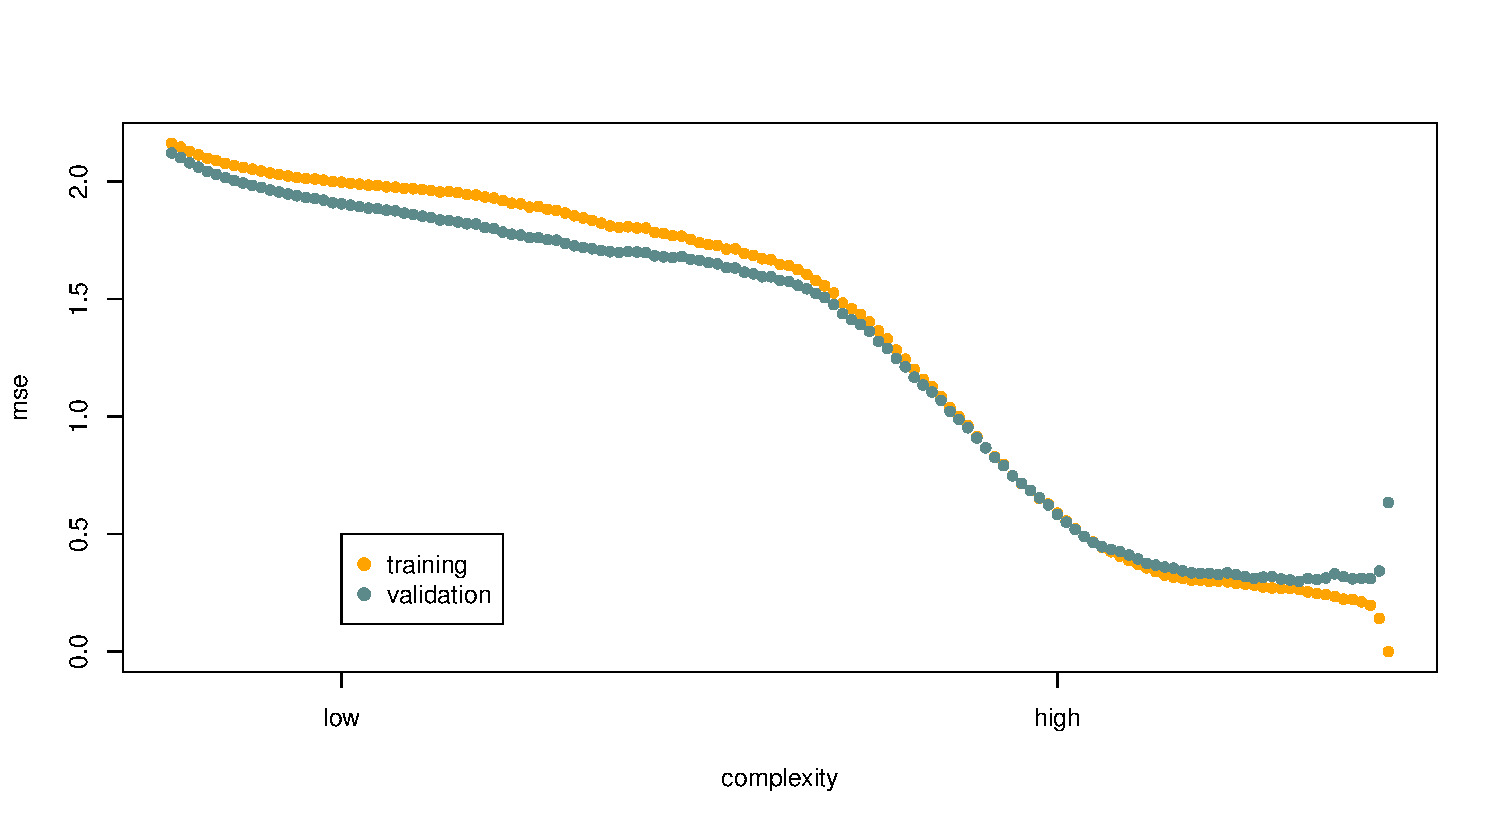
\includegraphics[width=\textwidth]{img/knnValid.pdf}
\end{center}

\end{frame}

%%%%%%%%%%%%%%%%%%%%%%%%%%%%%%%%%%%%%%%%%%%%%%%%%%%
\begin{frame}[fragile] \frametitle{} \oldB \small

\begin{center}
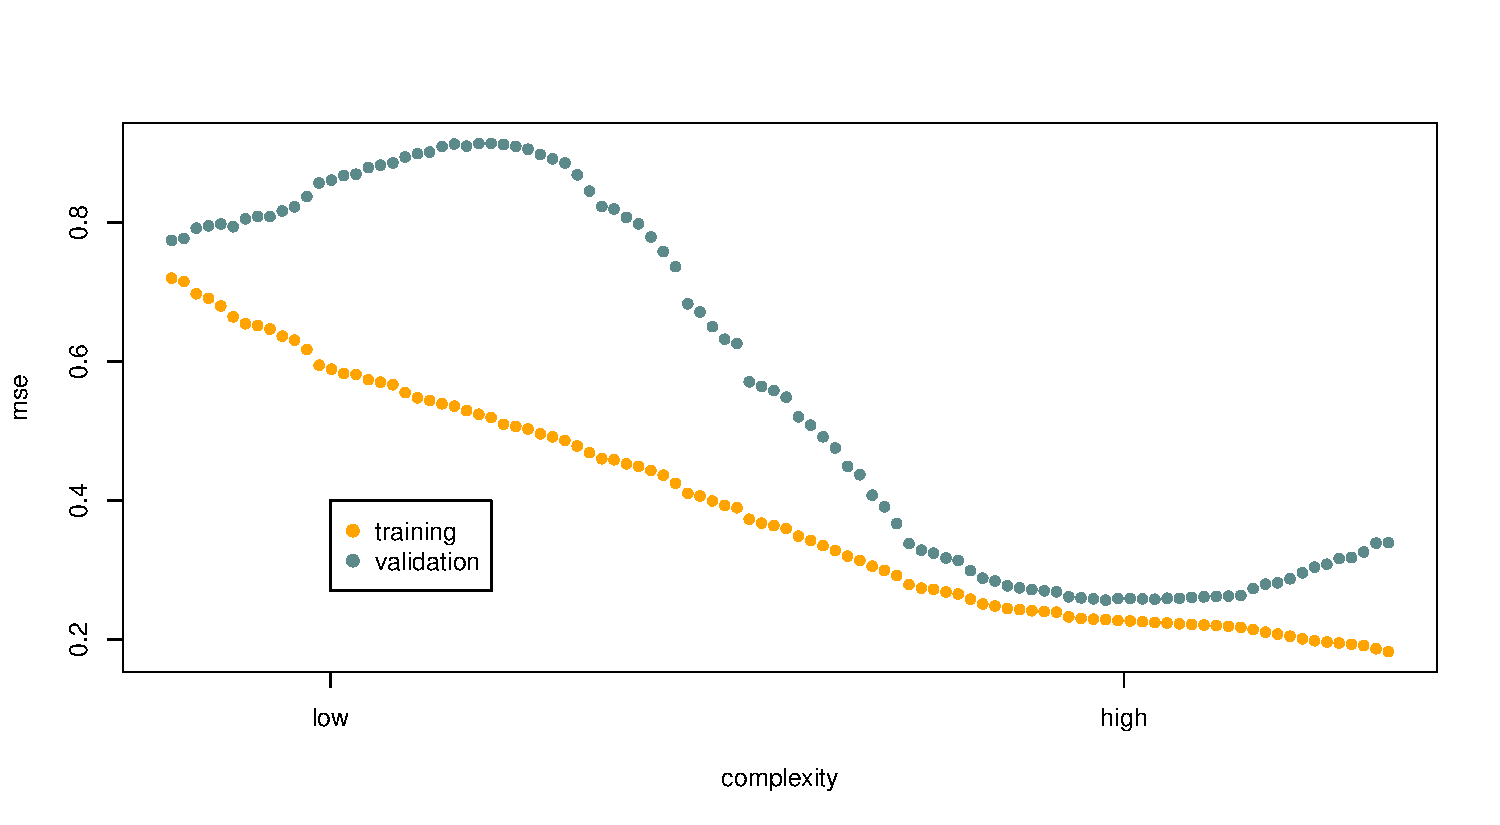
\includegraphics[width=\textwidth]{img/loessValid.pdf}
\end{center}

\end{frame}

%%%%%%%%%%%%%%%%%%%%%%%%%%%%%%%%%%%%%%%%%%%%%%%%%%%
\begin{frame}[fragile] \frametitle{} \oldB \small

\begin{center}
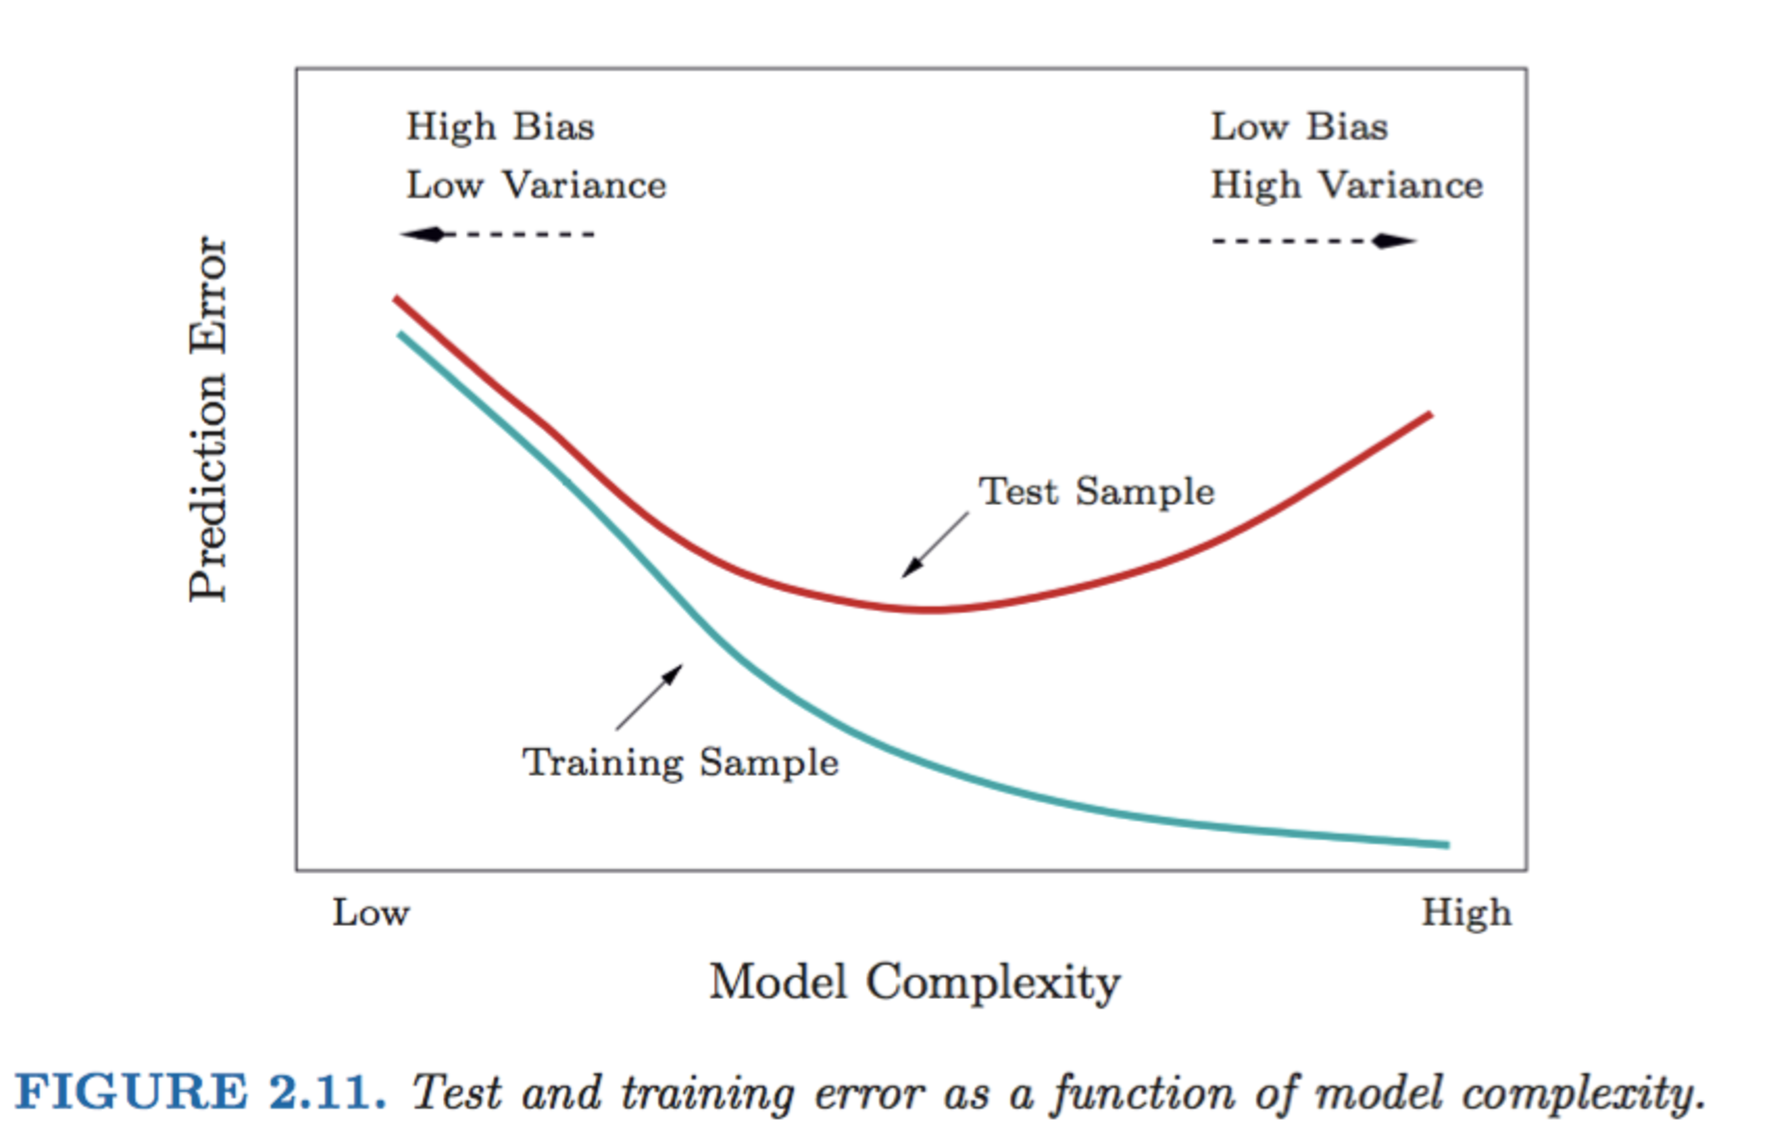
\includegraphics[width=0.7\textwidth]{img/pg38.pdf}
\end{center}

{\small \textbf{Elements of Statistical Learning, pg. 38}}

\end{frame}

%%%%%%%%%%%%%%%%%%%%%%%%%%%%%%%%%%%%%%%%%%%%%%%%%%%
\begin{frame}[fragile] \frametitle{} \oldB \small

\yblue{\textbf{Evaluating the model}}

Now, it seems that it is sufficient to divide our dataset into two
parts: testing and validation. However, we actually need a third
chunk of data called the \red{test set}. Once the tuning parameters
are selected based on the validation, we apply the model to the
test set to judge how well our algorithm has performed.

Why do we need to do this instead of just using the MSE on the
validation set?

\end{frame}

%%%%%%%%%%%%%%%%%%%%%%%%%%%%%%%%%%%%%%%%%%%%%%%%%%%
\begin{frame}[fragile] \frametitle{} \oldB \small

\begin{center}
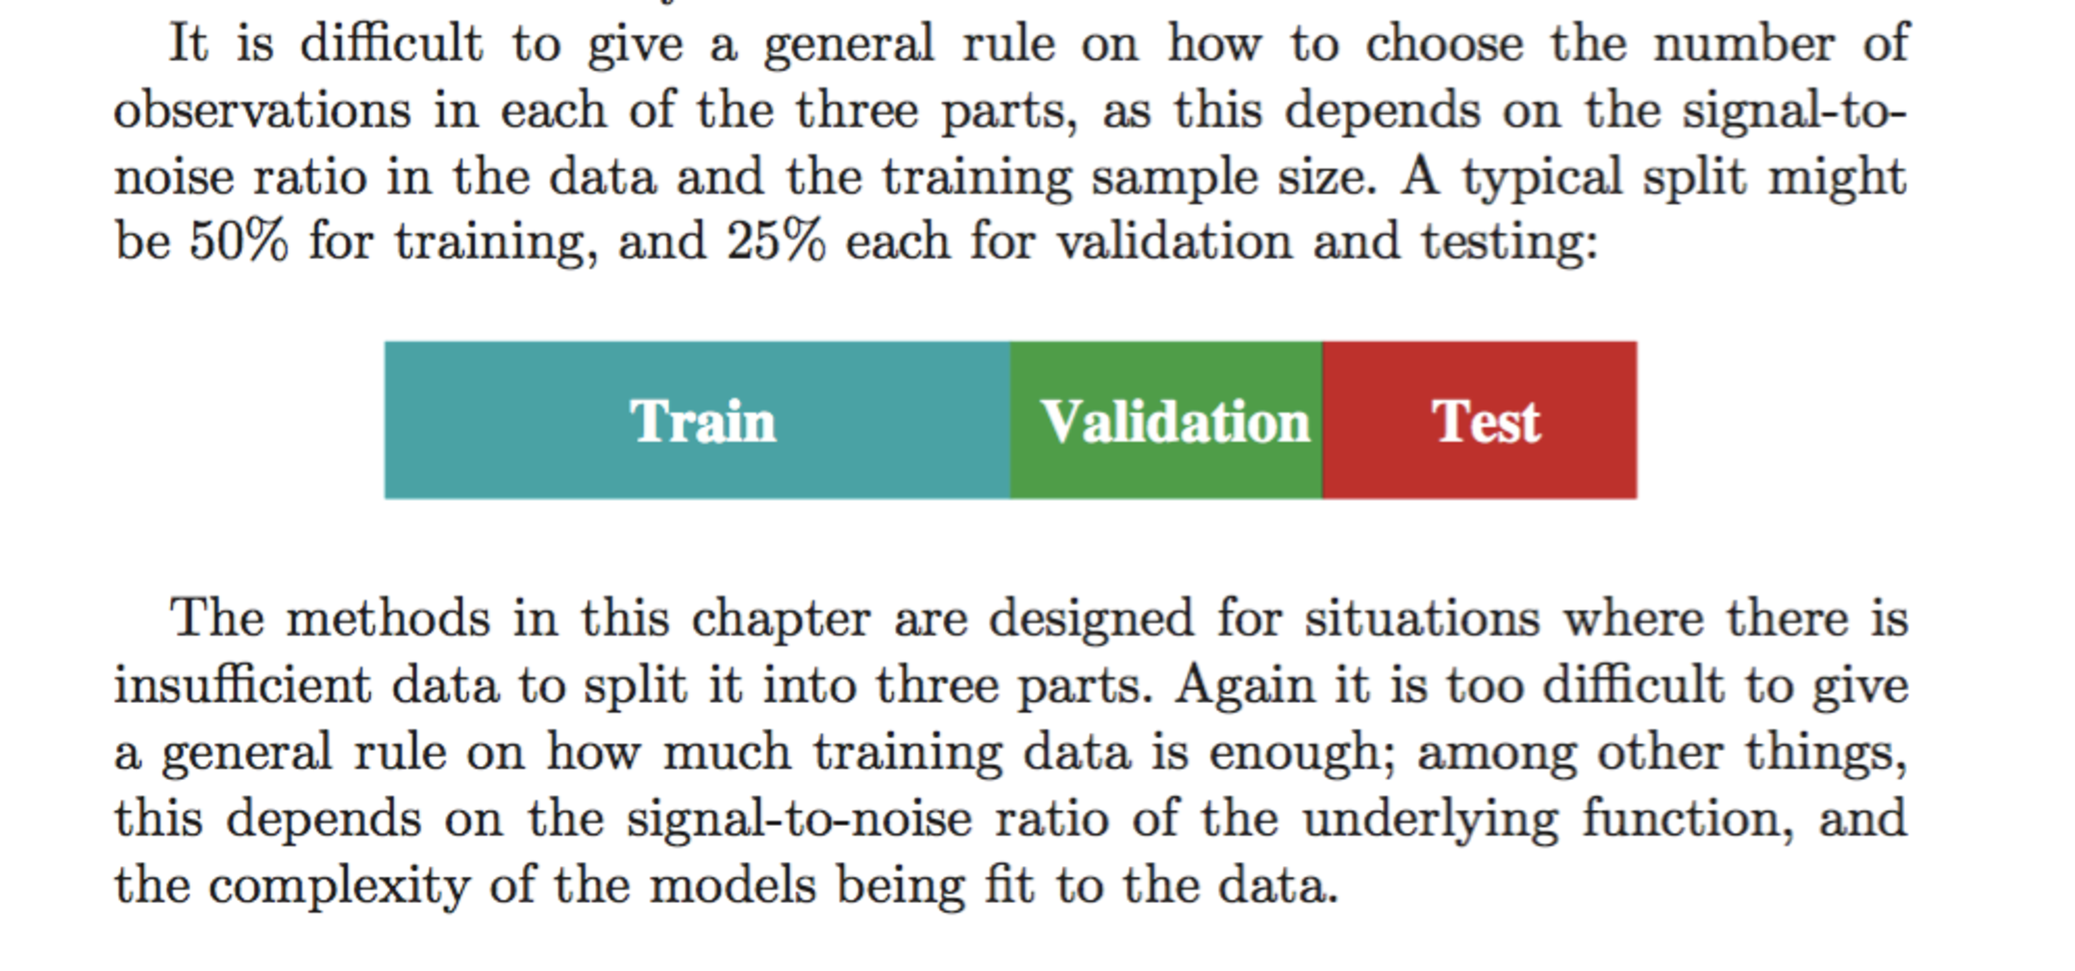
\includegraphics[width=\textwidth]{img/pg273.pdf}
\end{center}

{\small \textbf{Elements of Statistical Learning, pg. 273}}

\end{frame}

%%%%%%%%%%%%%%%%%%%%%%%%%%%%%%%%%%%%%%%%%%%%%%%%%%%
\begin{frame}[fragile] \frametitle{} \oldB \small

\yblue{\textbf{$k$-fold cross validation}}

We always need a fixed test set, but there is an alternative
to splitting the remainder of the data into distinct train
and validation buckets.

\pause Cross validation, or more specifically $k$-fold cross validation
instead:
\begin{enumerate}
\item randomly partitions the training set into $k$ equally sized
buckets
\item select one bucket to be the validation set and calculates the
MSE using the other $k-1$ buckets to train the data
\item then, selects a different bucket to the validation set and trains
on the remaining $k-1$ buckets
\item this is repeated $k$ times, until every observation has been in the
validation set once
\item the MSE for any value of the tuning parameter is calculated by averaging
the estimates across the $k$ runs
\end{enumerate}

\end{frame}

%%%%%%%%%%%%%%%%%%%%%%%%%%%%%%%%%%%%%%%%%%%%%%%%%%%
\begin{frame}[fragile] \frametitle{} \oldB \small

\begin{center}
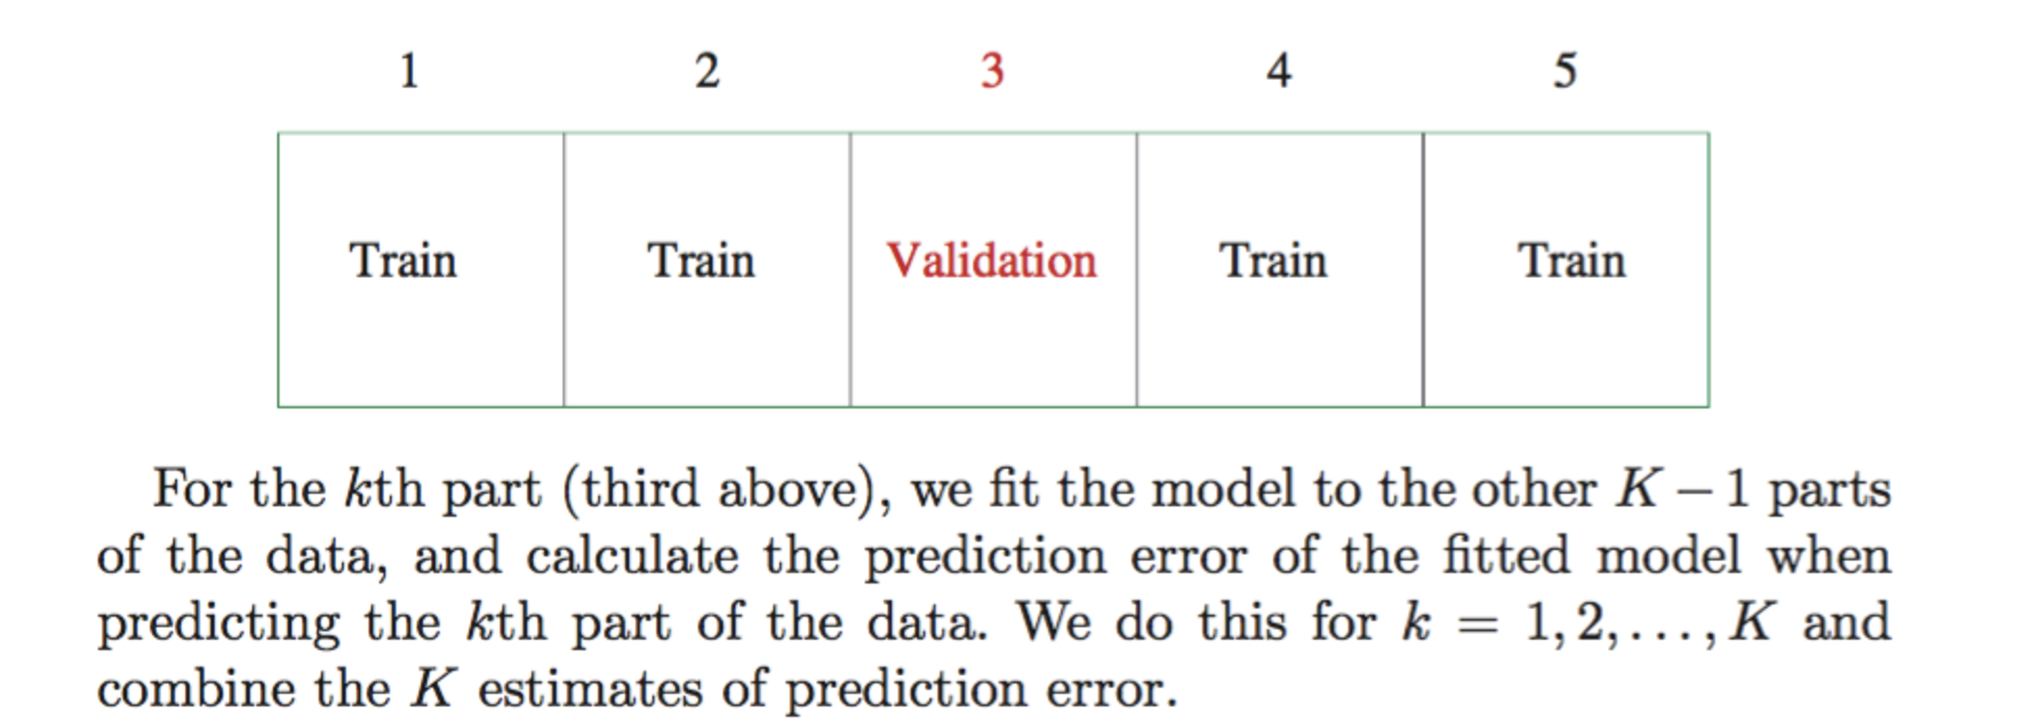
\includegraphics[width=\textwidth]{img/pg242.pdf}
\end{center}

{\small \textbf{Elements of Statistical Learning, pg. 242}}

\end{frame}

%%%%%%%%%%%%%%%%%%%%%%%%%%%%%%%%%%%%%%%%%%%%%%%%%%%
\begin{frame}[fragile] \frametitle{} \oldB \small

\begin{center}
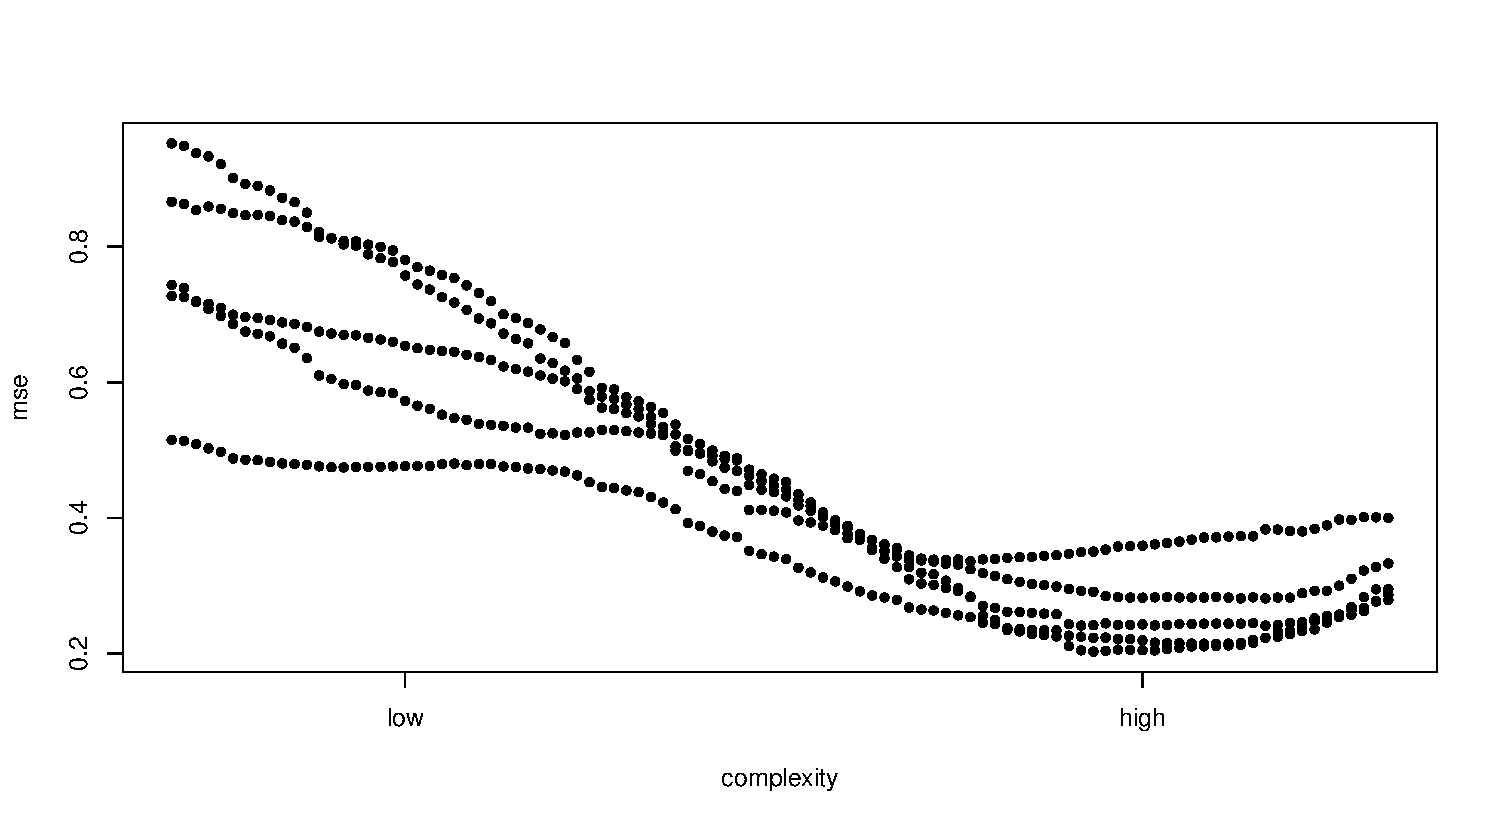
\includegraphics[width=\textwidth]{img/cv1.pdf}
\end{center}

\end{frame}

%%%%%%%%%%%%%%%%%%%%%%%%%%%%%%%%%%%%%%%%%%%%%%%%%%%
\begin{frame}[fragile] \frametitle{} \oldB \small

\begin{center}
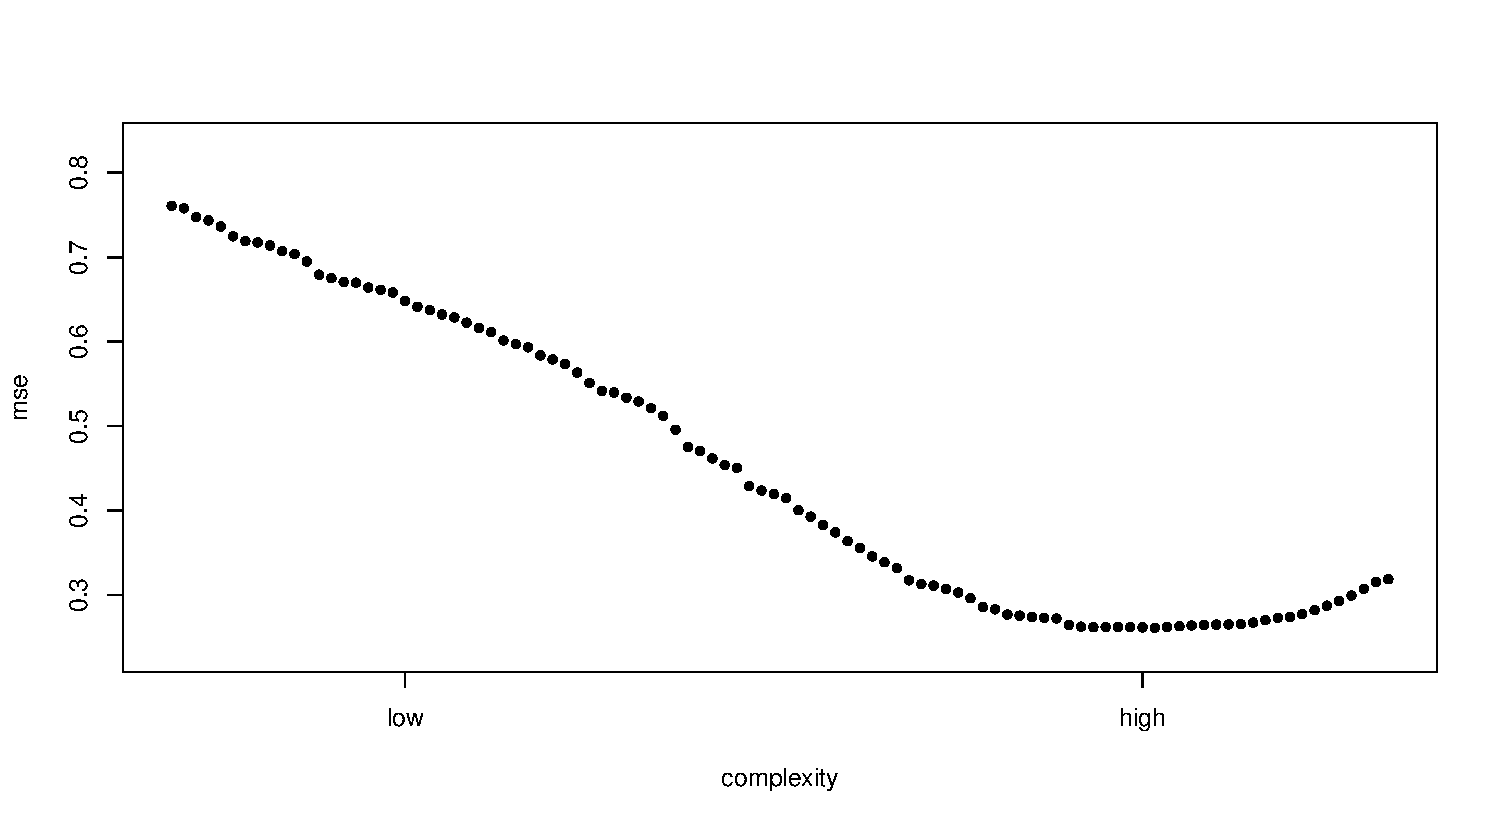
\includegraphics[width=\textwidth]{img/cv2.pdf}
\end{center}

\end{frame}

%%%%%%%%%%%%%%%%%%%%%%%%%%%%%%%%%%%%%%%%%%%%%%%%%%%
\begin{frame}[fragile] \frametitle{} \oldB \small

\begin{center}
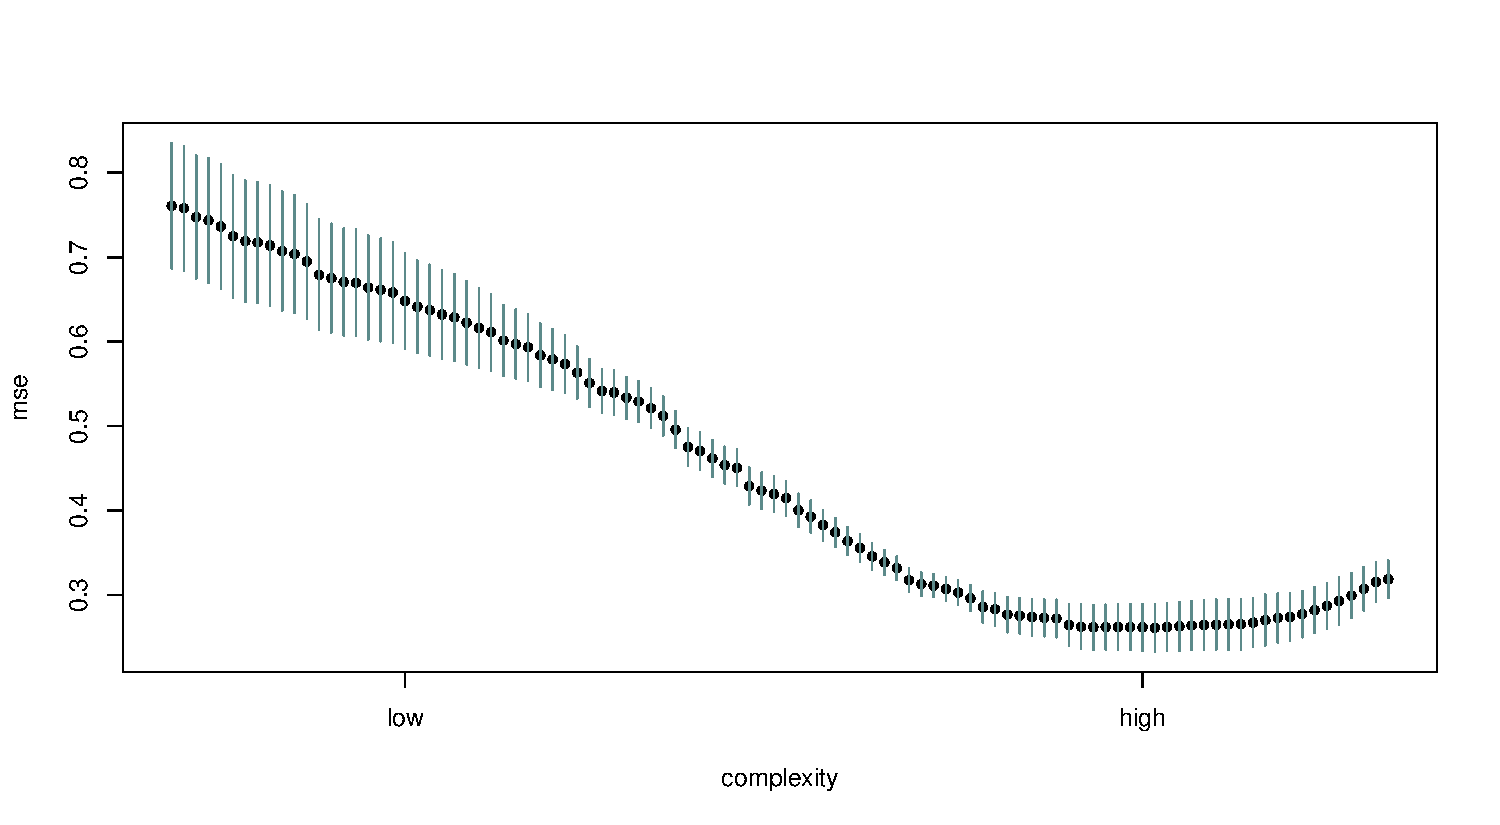
\includegraphics[width=\textwidth]{img/cv3.pdf}
\end{center}

\end{frame}

%%%%%%%%%%%%%%%%%%%%%%%%%%%%%%%%%%%%%%%%%%%%%%%%%%%
\begin{frame}[fragile] \frametitle{} \oldB \small

\begin{center}
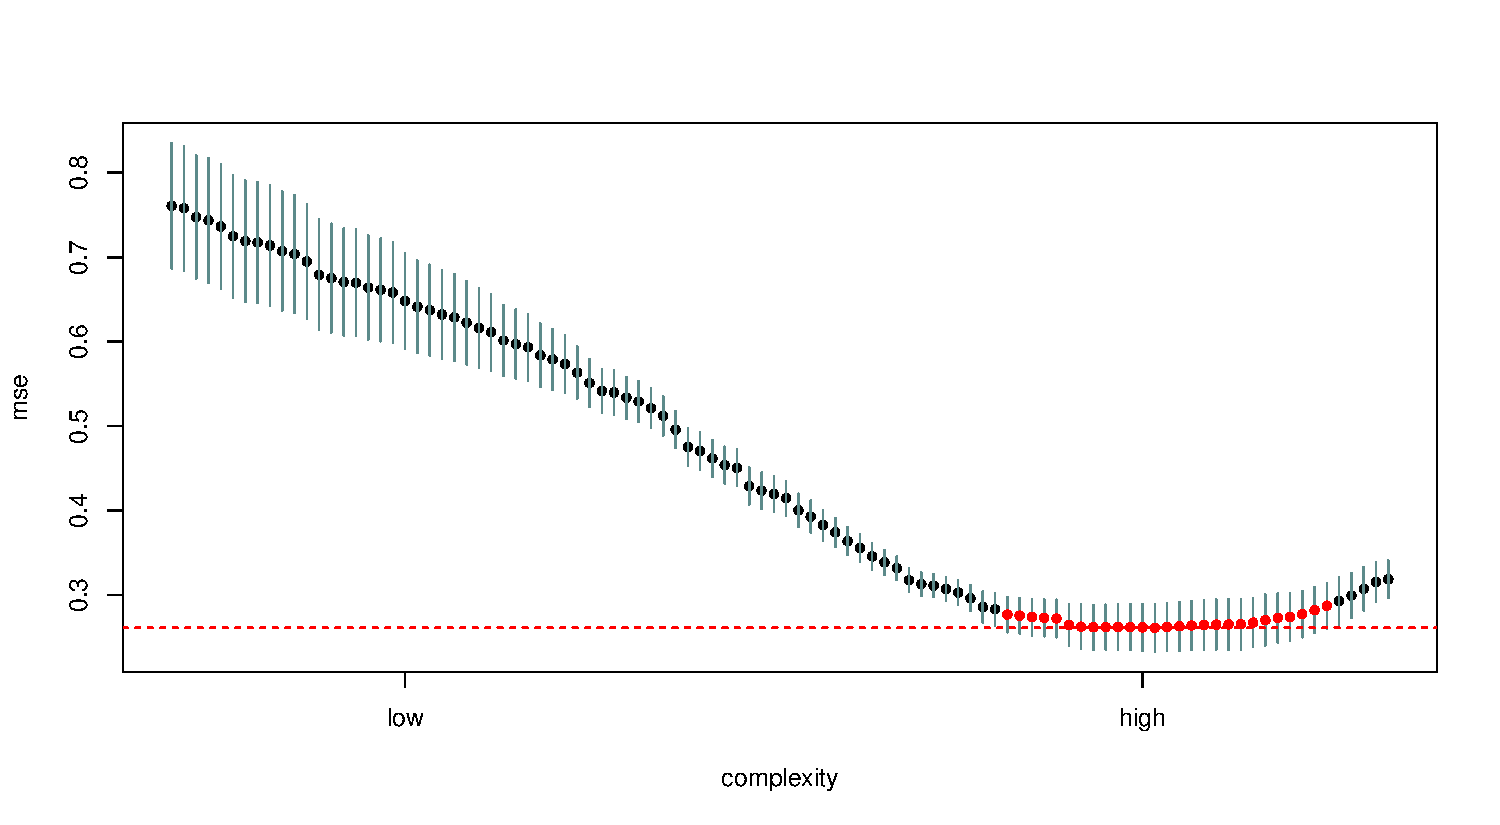
\includegraphics[width=\textwidth]{img/cv4.pdf}
\end{center}

\end{frame}


%%%%%%%%%%%%%%%%%%%%%%%%%%%%%%%%%%%%%%%%%%%%%%%%%%%
\begin{frame}[fragile] \frametitle{} \oldB \small

\yblue{\textbf{Still to come\ldots}}

\begin{itemize}
\item what happens when we have higher dimensional spaces
\item classification methods
\end{itemize}

\end{frame}



\end{document}













